\documentclass[tikz,border=10pt]{standalone}
\usepackage{xcolor}
\usepackage{tikz}
\usetikzlibrary{positioning, shapes.geometric, arrows.meta, shadows, calc}

\begin{document}
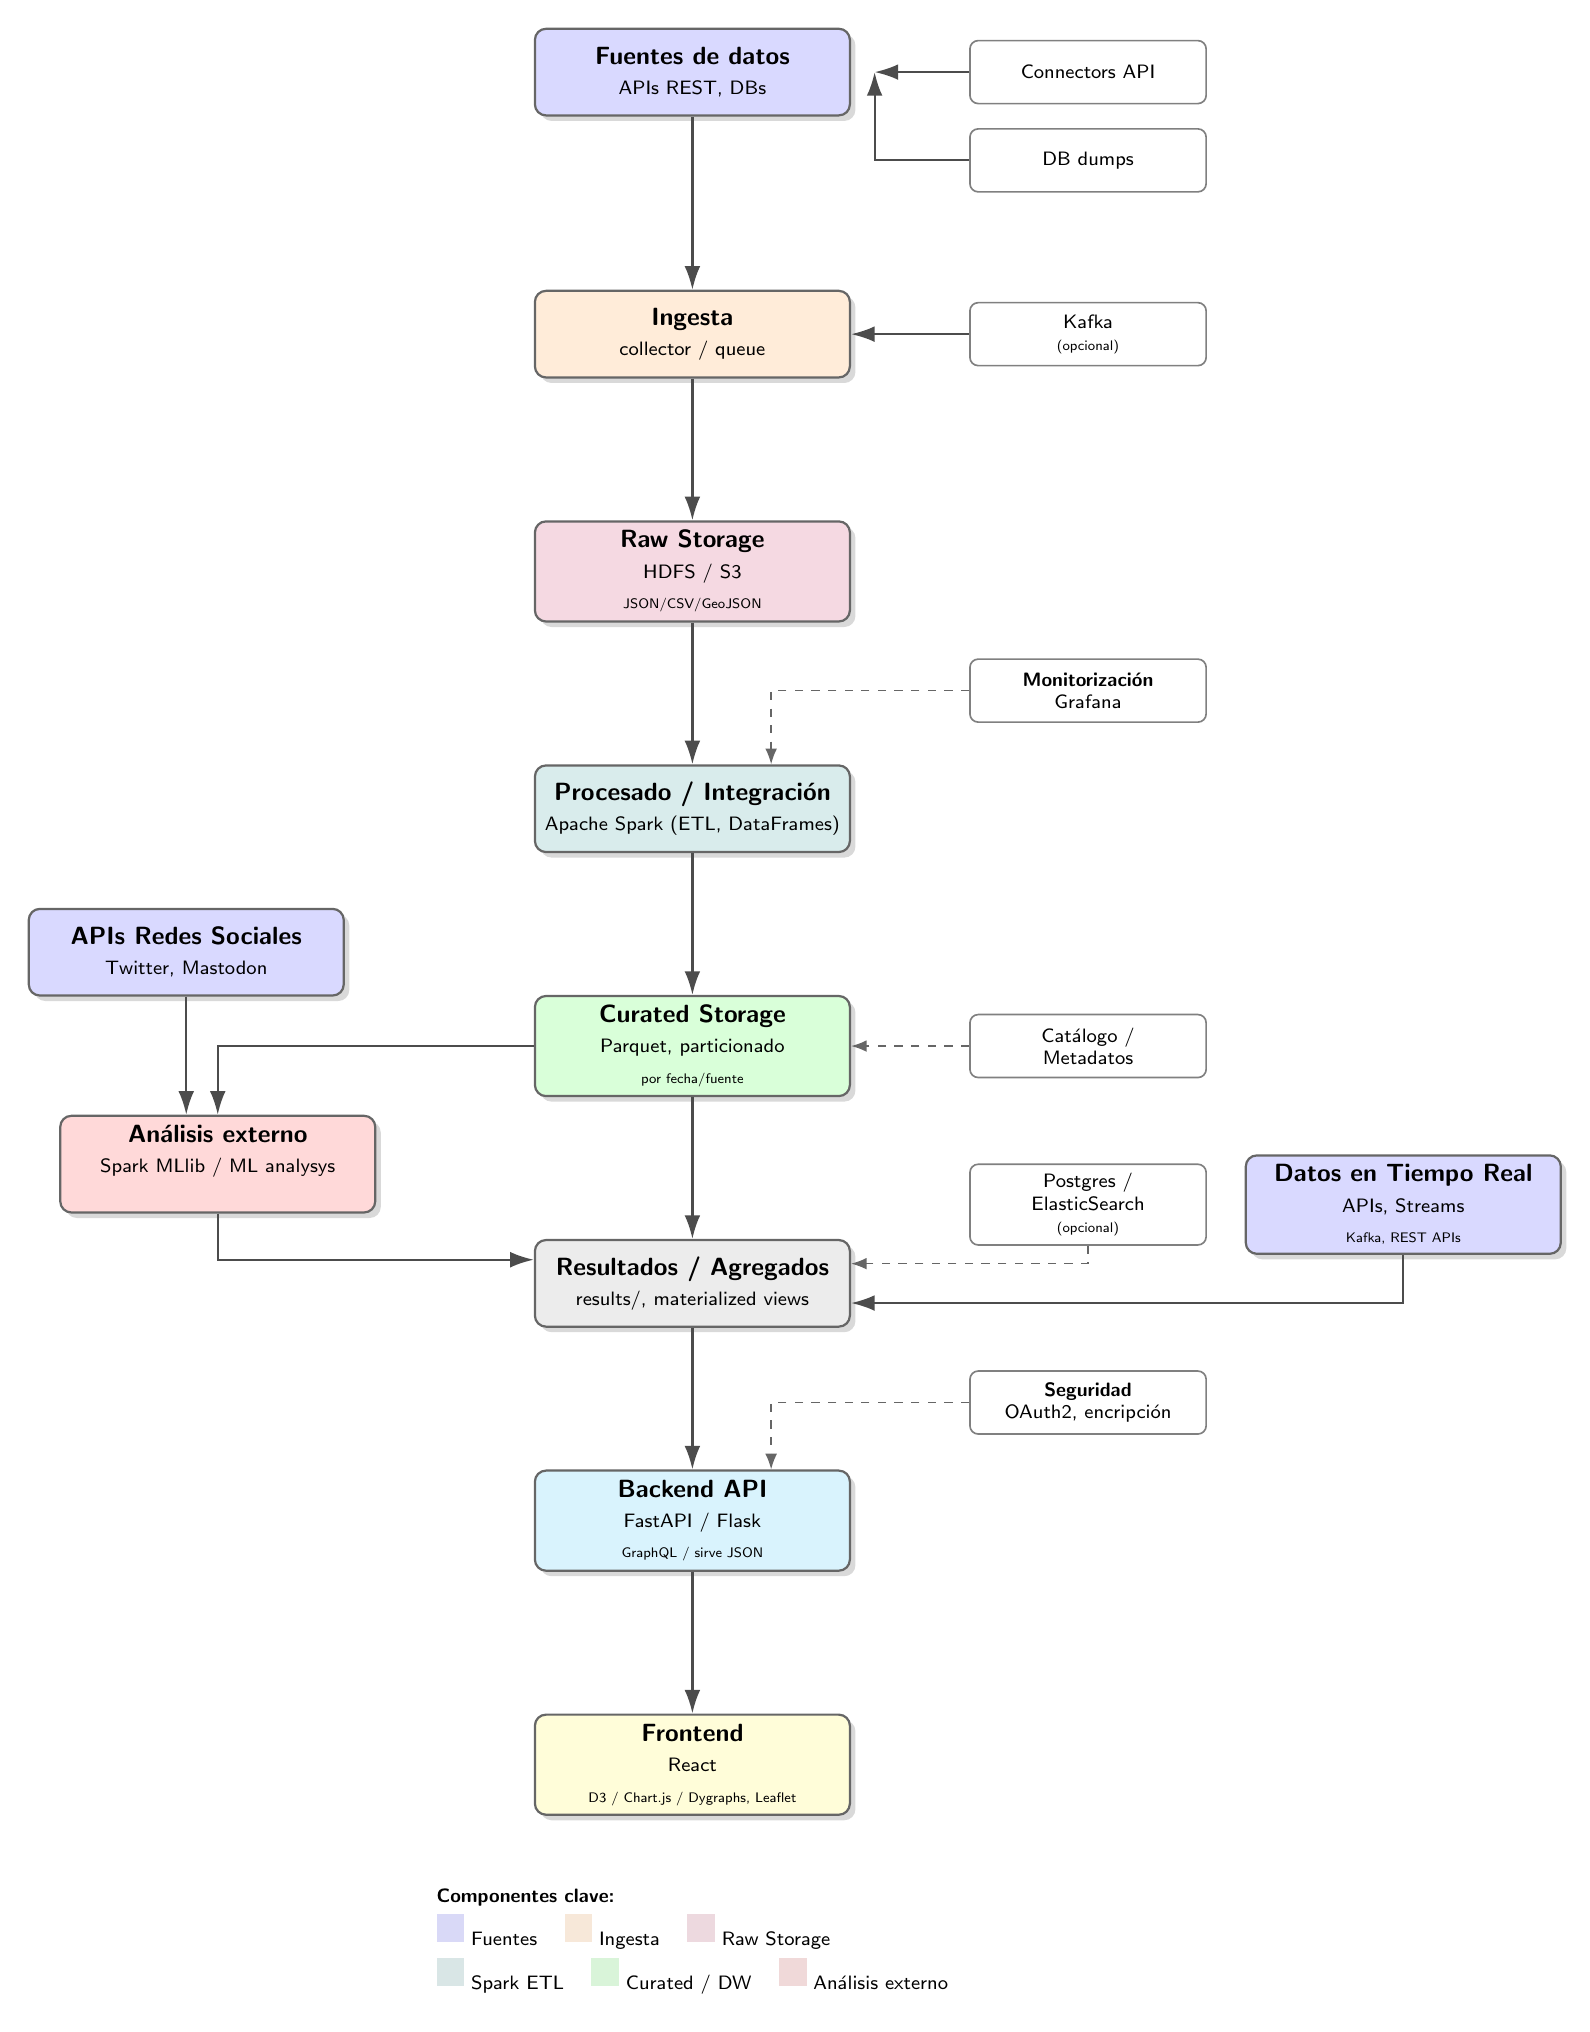
\begin{tikzpicture}[
  box/.style={
    rectangle, rounded corners=4pt, draw=black!60, fill=#1!15, 
    drop shadow={opacity=0.3, shadow xshift=2pt, shadow yshift=-2pt},
    minimum width=4cm, minimum height=1.1cm, align=center, 
    font=\small\sffamily, line width=0.8pt
  },
  comp/.style={
    rectangle, rounded corners=3pt, draw=black!50, fill=white, 
    minimum width=3cm, minimum height=0.8cm, align=center, 
    font=\scriptsize\sffamily, line width=0.6pt
  },
  arrow/.style={
    -{Latex[length=3mm,width=2mm]}, thick, draw=black!70
  },
  smallarrow/.style={
    -{Latex[length=2mm,width=1.5mm]}, semithick, draw=black!60, dashed
  }
]

% Layer 1: Data Sources
\node[box=blue] (sources) {\textbf{Fuentes de datos}\\{\scriptsize APIs REST, DBs}};
\node[comp, right=1.5cm of sources] (api) {Connectors API};
\node[comp, below=0.3cm of api] (db) {DB dumps};

% Layer 2: Ingestion
\node[box=orange, below=2.2cm of sources] (ingest) {\textbf{Ingesta}\\{\scriptsize collector / queue}};
\node[comp, right=1.5cm of ingest] (mq) {Kafka\\{\tiny (opcional)}};

% Layer 3: Raw Storage
\node[box=purple, below=1.8cm of ingest] (raw) {\textbf{Raw Storage}\\{\scriptsize HDFS / S3}\\{\tiny JSON/CSV/GeoJSON}};

% Layer 4: Processing
\node[box=teal, below=1.8cm of raw] (spark) {\textbf{Procesado / Integración}\\{\scriptsize Apache Spark (ETL, DataFrames)}};

% Layer 5: Curated Storage
\node[box=green, below=1.8cm of spark] (curated) {\textbf{Curated Storage}\\{\scriptsize Parquet, particionado}\\{\tiny por fecha/fuente}};
\node[comp, right=1.5cm of curated] (catalog) {Catálogo /\\Metadatos};

% Layer 6: Results
\node[box=gray, below=1.8cm of curated] (results) {\textbf{Resultados / Agregados}\\{\scriptsize results/, materialized views}};
\node[comp, right=1.5cm of results, yshift=1cm] (dbres) {Postgres /\\ElasticSearch\\{\tiny (opcional)}};

% Layer 7: Backend API
\node[box=cyan, below=1.8cm of results] (backend) {\textbf{Backend API}\\{\scriptsize FastAPI / Flask}\\{\tiny GraphQL / sirve JSON}};

% Layer 8: Frontend
\node[box=yellow, below=1.8cm of backend] (frontend) {\textbf{Frontend}\\{\scriptsize React}\\{\tiny D3 / Chart.js / Dygraphs, Leaflet}};

% Side: External Analysis (repositioned to avoid overlap)
\node[box=red, left=2cm of curated.west, yshift=-1.5cm] (analysis) {\textbf{Análisis externo}\\{\scriptsize Spark MLlib / ML analysys}\\{\tiny}};

% RealTime
\node[box=blue, right=5cm of results, yshift=1cm] (realtime) {\textbf{Datos en Tiempo Real}\\{\scriptsize APIs, Streams}\\{\tiny Kafka, REST APIs}};

% Social Media Api -> ML Analysis 
\node[box=blue, above=1.5cm of analysis, xshift=-0.4cm] (social) {\textbf{APIs Redes Sociales}\\{\scriptsize Twitter, Mastodon}};

\draw[arrow] (social.south) -- ($(analysis.north) + (-0.4,0)$);

% Side: Monitoring & Security (repositioned)
\node[comp, right=1.5cm of spark.east, yshift=1.5cm] (monitor) {\textbf{Monitorización}\\Grafana};
\node[comp, right=1.5cm of backend.east, yshift=1.5cm] (security) {\textbf{Seguridad}\\OAuth2, encripción};

% Main vertical flow
\draw[arrow] (sources) -- (ingest);
\draw[arrow] (ingest) -- (raw);
\draw[arrow] (raw) -- (spark);
\draw[arrow] (spark) -- (curated);
\draw[arrow] (curated) -- (results);
\draw[arrow] (results) -- (backend);
\draw[arrow] (backend) -- (frontend);

% Component connections (right side)
\draw[arrow] (api.west) -- ($(sources.east) + (0.3,0)$);
\draw[arrow] (db.west) -| ($(sources.east) + (0.3,0)$);

\draw[arrow] (mq.west) -- (ingest.east);

% Analysis flow (improved routing)
\draw[arrow] (curated.west) -| (analysis.north);
\draw[arrow] (analysis.south) |- ($(results.west) + (0,0.3)$);

% Auxiliary connections
\draw[smallarrow] (catalog.west) -- (curated.east);
\draw[smallarrow] (dbres.south) |- ($(results.east) + (0,0.25)$);
\draw[arrow] (realtime.south) |- ($(results.east) - (0,0.25)$);
\draw[smallarrow] (monitor.west) -| ($(spark.north) + (1,0)$);
\draw[smallarrow] (security.west) -| ($(backend.north) + (1,0)$);

% Legend
\node[align=left, font=\scriptsize\sffamily, below=0.8cm of frontend] (legend) {
  \textbf{Componentes clave:}\\[2pt]
  \raisebox{0.5ex}{\tikz \fill[blue!80!black!15] (0,0) rectangle (0.35,0.35);} Fuentes \quad
  \raisebox{0.5ex}{\tikz \fill[orange!80!black!15] (0,0) rectangle (0.35,0.35);} Ingesta \quad
  \raisebox{0.5ex}{\tikz \fill[purple!70!black!15] (0,0) rectangle (0.35,0.35);} Raw Storage\\[2pt]
  \raisebox{0.5ex}{\tikz \fill[teal!70!black!15] (0,0) rectangle (0.35,0.35);} Spark ETL \quad
  \raisebox{0.5ex}{\tikz \fill[green!70!black!15] (0,0) rectangle (0.35,0.35);} Curated / DW \quad
  \raisebox{0.5ex}{\tikz \fill[red!60!black!15] (0,0) rectangle (0.35,0.35);} Análisis externo
};

\end{tikzpicture}
\end{document}